% !TeX root = ..

\section{
  Технологии и техники листовой резки
  на~машинах с~ЧПУ
}
\label{sect:1.1}
\setcounter{equation}{0}

В машиностроении,
производстве металлоконструкций
и других отраслях промышленности существенная часть продукции
изготавливается из заготовок,
получаемых из листовых материалов на различном технологическом оборудовании.
К такому оборудованию относятся, в частности,
используемые на предприятиях отечественные и зарубежные
системы автоматизированного проектирования (САПР),
предназначенные для разработки управляющих программ (УП)
для машин листовой резки с ЧПУ
(т. н. \textit{Computer-Aided Manufacturing},
\textit{CAM}-системы),
которые
обеспечивают автоматизацию процесса разработки УП,
однако не позволяют решить многие оптимизационные задачи.
При этом при моделировании маршрута инструмента пользователям
САПР часто приходится применять интерактивные методы проектирования УП,
поскольку алгоритмы генерации УП,
реализованные в автоматическом режиме проектирования,
во многих случаях не позволяют генерировать оптимальные управляющие программы,
а также обеспечить соблюдение некоторых технологических требований листовой резки.
В качестве критериев оптимизации имеются в виду время резки и
некоторые другие стоимостные характеристики процесса листовой резки.
Проблема разработки методов, алгоритмов и соответствующего программного обеспечения,
позволяющих в автоматическом режиме оптимизировать параметры
процесса резки заготовок из листовых материалов на машинах с ЧПУ,
включая алгоритмы маршрутизации движения инструмента,
которые бы обеспечивали минимизацию времени резки и стоимости процесса,
остается актуальнейшей задачей раскройно-заготовительного производства.

Рассмотрим понятие маршрута инструмента (маршрута резки)
применительно к некоторым технологиям фигурной листовой резки.
В настоящее время в промышленном производстве
единичного и мелкосерийного типа для раскроя листовых материалов
используются в основном следующие технологии:
лазерная, плазменная, газовая и гидроабразивная.
Целесообразность их применения определяется различными технологическими факторами,
например, свойствами раскраиваемого материала,
экономическими требованиями к процессу резки,
требованиями к качеству реза и пр.
Эти и некоторые другие технологии резки предполагают,
что для сохранения требуемой геометрии заготовки
траектория движения режущего инструмента не совпадает
с граничным контуром заготовки,
а задается некоторой эквидистантой этого контура,
поскольку часть материала вырезается (<<сгорает>>, <<вымывается>> и пр.)
в процессе резки.
Как правило, дистанция между эквидистантным контуром,
по которому осуществляется резка, и граничным контуром заготовки определяется величиной,
равной половине ширины реза.
Эта величина зависит от выбранной технологии резки,
толщины и марки материала, заданной скорости резки
и особенностей конкретного технологического оборудования,
используемого для резки.

Еще одна особенность листовой резки –
необходимость предварительной врезки (пробивки)
материала перед процессом резки непосредственно
по эквидистантному контуру заготовки.
Пробивка материала сопровождается дополнительными
деформациями материала в точке врезки,
поэтому производится на расстоянии (дистанции)
от контура заготовки большем,
чем дистанция до эквидистантного контура за исключением случаев,
когда для точек врезки в листовом материале механическим способом
готовятся (например, просверливаются)
отверстия.
Врезка может также осуществляться
непосредственно на границе материала
(<<врезка с края листа>>).
В этом случае достигается уменьшение
деформаций материала и сокращается время врезки.

На рис. \ref{standard-cutting}.
показан
один из способов резки заготовки
(стандартная техника).

\begin{figure}[h]
  \begin{center}
  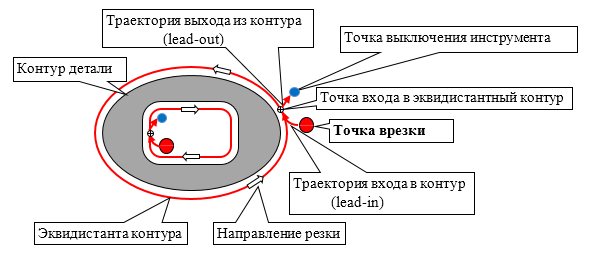
\includegraphics[width=0.9\textwidth]{cutting-path.png}
  \caption{Схема стандартной техники резки (резка по замкнутому контуру)}
  \label{standard-cutting}
  \end{center}
\end{figure}

Если используется стандартная техника резки,
то в этом случае каждый замкнутый контур вырезается целиком,
и после резки одного контура переход к следующей точке врезки
происходит с выключенным инструментом на холостом ходу.
При этом точка выключения инструмента
в общем случае
может не совпадать с точкой входа в эквидистантный контур заготовки,
по которому осуществляется резка, и также,
как и точка врезки,
может лежать вне заданного эквидистантного контура.
Во многих случаях допускается программирование точки выключения
инструмента непосредственно на эквидистантном контуре.

Стратегия минимизации тепловых деформаций при термической резке
и требования к качеству реза порождают необходимость управления
не только выбором точек врезки,
но и управлением траекторией подхода к контуру
(\textit{lead-in})
и способом выхода из контура
(\textit{lead-out}).
В зависимости от конкретных условий
(вида термической резки, марки и толщины материала,
скорости резки, геометрической формы контура и пр.)
подход к контуру может осуществляться по дуге окружности,
касательная к которой совпадает с касательной к контуру в точке входа,
либо производиться по прямой линии
(например, по наикратчайшему расстоянию до контура).
Соответственно и после завершения резки выход из контура
также может осуществляться с включенным инструментом
(либо по дуге, либо по прямой линии).
Необходимость выхода из контура с включенным
инструментом может быть вызвана тем,
что в точке выключения инструмента может возникнуть
<<вырыв>> или оплавление части материала,
что приводит к искажению геометрии заготовки.
Уменьшение эффекта деформации заготовок обеспечивает
также врезка в <<угловые>> точки заготовок
(рис.~\ref{corner}).

\begin{figure}[h]
  \begin{center}
  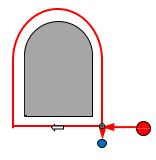
\includegraphics[width=0.45\textwidth]{corner.png}
  \caption{Пример врезки <<в угол>>}
  \label{corner}
  \end{center}
\end{figure}

Примером нестандартной техники
может служить <<цепная>> резка,
которая заключается в резке нескольких контуров с
использованием одной точки врезки.
При этом каждый контур,
как и в случае применения стандартной техники резки,
вырезается целиком.
На рис.~\ref{chain}
показан пример схемы резки двух заготовок,
в которой резка внешних контуров обеих заготовок
производится без выключения инструмента
с использованием только одной точки врезки.

Перемещение инструмента в точку врезки
в этом примере начинается из начальной точки на холостом ходу,
а после завершения резки последнего контура
предусмотрен возврат инструмента в начальную точку.

\begin{figure}[h]
  \begin{center}
  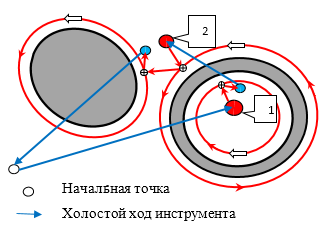
\includegraphics[width=0.65\textwidth]{chain.png}
  \caption{
    Пример схемы резки двух заготовок
    с~использованием стандартной
    и~<<цепной>> техники резки}
  \label{chain}
  \end{center}
\end{figure}

На практике применяется также техника резки
замкнутого контура заготовок по частям
с использованием нескольких точек врезки
с целью формирования т. н. <<перемычек>>
(рис.~\ref{jumper}),
а также используются другие специальные приемы,
целью которых является оптимизация различных параметров,
характеризующих процесс резки,
и соблюдение необходимых технологических требований резки.
Техника резки <<перемычка>> предусматривает
оставление невырезанной части контура заготовки,
обычно небольшого прямолинейного отрезка или нескольких отрезков
с резкой этих отрезков после завершения резки оставшейся части контура.
Этот прием применяется с целью уменьшения деформаций материала
при термической резке заготовок, склонных к термическим деформациям,
в частности, длинномерных заготовок.

\begin{figure}[h]
  \begin{center}
  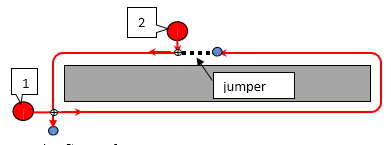
\includegraphics[width=0.75\textwidth]{jumper.png}
  \caption{Схема формирования перемычки на контуре при резке полосы}
  \label{jumper}
  \end{center}
\end{figure}

На рис.~\ref{saber} показан пример искажения геометрической формы
(получения т. н. формы <<сабли>>)
и~изменения размера длинномерной прямоугольной заготовки,
вырезаемой без использования техники <<перемычка>>.

\begin{figure}[h]
  \begin{center}
  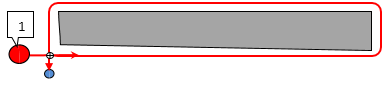
\includegraphics[width=0.75\textwidth]{saber.png}
  \caption{
    Результат изменнения формы
    и~размера прямоугольной заготовки
    при~термической резке
    }
  \label{saber}
  \end{center}
\end{figure}

На рис.~\ref{bridge}
приведен пример использования техники <<мост>>,
предполагающей  частичную резку замкнутого контура
заготовки с последующим завершением резки контура
после резки контура другой заготовки или
группы контуров других заготовок.
Эта техника используется при резке двух или
нескольких рядом расположенных заготовок и
предусматривает переход по короткой траектории (<<мосту>>)
к резке другой заготовки и возврат к первому контуру
по этой же траектории для завершения процесса резки.
Так же, как и <<перемычки>>,
мосты существенно уменьшают тепловые деформации материала,
особенно при резке длинномерных заготовок,
кроме того, сокращают число точек врезки.

\begin{figure}[h]
  \begin{center}
  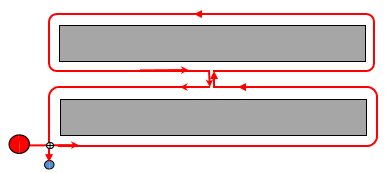
\includegraphics[width=0.75\textwidth]{bridge.png}
  \caption{Схема резки двух полос с использованием техники <<мост>>}
  \label{bridge}
  \end{center}
\end{figure}

Разновидностью техники <<мост>> можно считать технику <<змейка>>,
показанную на рис.~\ref{snake},
в которой также используется прием
частичной резки контура и резки
нескольких заготовок без выключения инструмента.

\begin{figure}[h]
  \begin{center}
  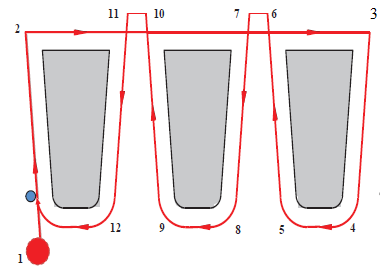
\includegraphics[width=0.85\textwidth]{snake.png}
  \caption{Схема резки <<змейка>>}
  \label{snake}
  \end{center}
\end{figure}

Для уменьшения длины рабочего хода инструмента
применяют т. н. <<совмещенный>> рез.
Он используется для вырезки заготовок,
которые содержат прямолинейные отрезки в контуре
и которые в процессе раскроя размещаются таким образом,
что имеют общую границу по одному из таких прямолинейных отрезков.
Общая прямолинейная граница позволяет размещать
заготовки с половинным припуском на рез
(т. е. на ширину реза),
поскольку режется только один раз,
что экономит материал и сокращает суммарную
длину резки на величину совмещенного реза.
Совмещенный рез реализован, в частности,
в технике резки <<восьмерка>>,
применяемой для резки двух одинаковых заготовок
(рис.~\ref{8}).
В этой технике используется также идея цепной резки.

\begin{figure}[h]
  \begin{center}
  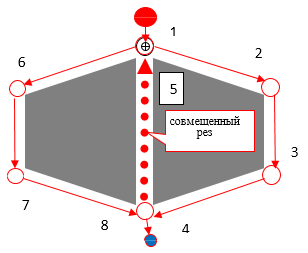
\includegraphics[width=0.6\textwidth]{8.png}
  \caption{Схема резки <<восьмеркой>> двух заготовок}
  \label{8}
  \end{center}
\end{figure}

Основные технологические требования
фигурной резки на машинах с ЧПУ обусловлены
необходимостью учета возникающих деформаций
материала и искажения геометрических размеров
вырезаемых заготовок при использовании
термических технологий резки.
Применение специальных техник позволяет
уменьшить эффект искажения геометрии,
который особенно значителен при
использовании газовой и плазменной технологий.

При использовании любой техники резки маршрут инструмента
машины с ЧПУ для фигурной листовой резки
включает в себя следующие компоненты:
\begin{itemize}
  \item точки врезки;
  \item рабочий ход инструмента;
  \item точки выключения инструмента;
  \item линейное перемещение инструмента на холостом ходу
  между точкой выключения инструмента и следующей точкой врезки.
\end{itemize}

При разработке управляющей программы
первое перемещение инструмента обычно
программируется, как на рис.~\ref{chain},
из начальной точки.

Отметим, что некоторые машины фигурной листовой
резки с ЧПУ могут быть укомплектованы
специальным видом инструмента,
т. н. трехрезаковым блоком для вырезания
из листа заготовок с одновременной разделкой
кромок поверхности реза для последующей сварки.
Врезка в материал для такого инструмента
программируется специальными способами.

Введем некоторые определения,
касающиеся понятия маршрута резки.
В дальнейшем при формальном обозначении
математических и геометрических категорий
мы будем использовать стандартную
теоретико-множественную символику.
Ее детальное описание дано в
\ref{sect:3.1}.
Введем следующее определение.

\begin{opred}
\label{def:cutting-segment}
{\bf Сегментом резки}
$S=MM^*$
будем называть траекторию рабочего хода
инструмента между точкой врезки
$M$
и соответствующей ей точкой выключения инструмента
$M^*$.
Геометрически сегмент резки представляет собой
определенную на эвклидовой плоскости
$\mathbb R \times \mathbb R$
кривую.
$(S \subset \mathbb R \times \mathbb R;
M=(x,y) \in \mathbb R \times \mathbb R,
M^* =(x^*,y^*)\in \mathbb R \times \mathbb R)$.
Будем также полагать,
что в каждой точке траектории определено направление движения инструмента.
Заметим, что если сегмент резки не содержит замкнутых контуров,
то направление движения резки в каждой точке траектории
однозначно определяется начальной точкой сегмента
(точкой врезки).
Замкнутые контуры в траектории рабочего хода инструмента
могут появляться не только в результате резки контуров заготовок,
но и при программировании т. н. петель,
которые используются для повышения качества реза.
\end{opred}

Используя понятие сегмента резки,
все техники фигурной резки на машинах с ЧПУ
можно разделить на три класса.
\begin{enumerate}
  \item
  {\it Резка по замкнутому контуру (стандартная техника)}:
  в этом случае сегмент резки содержит
  ровно один замкнутый эквидистантный контур заготовки,
  который вырезается целиком.
  \item
  {\it Мультисегментная резка контура}:
  в этом случае для вырезки одного контура
  используются не менее двух сегментов резки.
  \item
  {\it Мультиконтурная резка}:
  резка предполагает вырезку нескольких
  контуров в одном сегменте.
\end{enumerate}

Примерами мультиконтурной резки являются,
в частности, приведенные выше техники резки:
<<цепная резка>>, <<мост>>, <<змейка>> и <<восьмерка>>,
а примером мультисегментной резки --
резка с перемычкой.
На практике используются и другие специальные техники резки,
но все они являются разновидностями техник,
относящихся к одному из определенных выше классов.

При разработке управляющих программ для
машин фигурной листовой резки с ЧПУ чаще всего
применяется стандартная техника резки.
Вместе с тем нередко используются и
комбинации различных техник резки.
Применение той или иной техники резки
при проектировании маршрута резки в
каждом конкретном случае, как правило,
обусловлено либо технологическими требованиями резки,
либо стремлением оптимизировать некоторые
параметры листовой резки.
Подробнее эти вопросы рассмотрены ниже.
